% ------------------------------------------------------------------ %
% Examination of a Bayesian approach to inverse kinematics.
% Andrew J. Pohl, Matthew R. Schofield & Reed Ferber
% Submitted to Journal of Biomechanics March 2021
% SupplementaryMaterialA.tex
% ------------------------------------------------------------------ %
\documentclass{article}
\usepackage{setspace}

% ------------------------------------------------------------------ %
% Examination of a Bayesian approach to inverse kinematics.
% Andrew J. Pohl, Matthew R. Schofield & Reed Ferber
% Submitted to Journal of Biomechanics March 2021
% SupplementaryMaterial Structure
% structure.tex
% ------------------------------------------------------------------ %
%% Package inclusion
\usepackage[running]{lineno} % Line Numbers


 \usepackage[authoryear]{natbib}
\bibliographystyle{model5-names}

% SI 
\usepackage{siunitx}
% Hyper refferences
\usepackage{hyperref}

% Packages for tables
\usepackage{multirow}

% Packages for figures
\usepackage{subcaption}	

% Math Packages
\usepackage{amsmath,amsfonts,stmaryrd,amssymb, bm} 
\DeclareMathOperator*{\argmin}{argmin} 

\usepackage{enumerate} % Custom item numbers for enumerations

\usepackage[ruled]{algorithm2e} % Algorithms

\usepackage[framemethod=tikz]{mdframed} % Allows defining custom boxed/framed environments

\usepackage{listings} % File listings, with syntax highlighting
\lstset{
	basicstyle=\ttfamily, % Typeset listings in monospace font
}

%----------------------------------------------------------------
%	DOCUMENT MARGINS
%----------------------------------------------------------------

\usepackage{geometry} % Required for adjusting page dimensions and margins

\geometry{
	paper=letterpaper, % Paper size, change to letterpaper for US letter size
	top=2.5cm, % Top margin
	bottom=3cm, % Bottom margin
	left=2.5cm, % Left margin
	right=2.5cm, % Right margin
	headheight=14pt, % Header height
	footskip=1.5cm, % Space from the bottom margin to the baseline of the footer
	headsep=1.2cm, % Space from the top margin to the baseline of the header
	%showframe, % Uncomment to show how the type block is set on the page
}

%-------------------------------------------------------------------------
%	FONTS
%-------------------------------------------------------------------------

\usepackage[utf8]{inputenc} % Required for inputting international characters
\usepackage[T1]{fontenc} % Output font encoding for international characters

\usepackage{XCharter} % Use the XCharter fonts

%---------------------------------------------------------------------------
%	EMPHASISE ENVIRONMENT
%---------------------------------------------------------------------------

% Usage:
% \begin{emphasise}
%	\begin{verbatim}
%		$ ls
%		
%		Applications	Desktop	...
%	\end{verbatim}
% \end{commandline}

\mdfdefinestyle{emphasise}{
	leftmargin=10pt,
	rightmargin=10pt,
	innerleftmargin=15pt,
	middlelinecolor=black!50!white,
	middlelinewidth=2pt,
	frametitlerule=false,
	backgroundcolor=black!5!white,
	frametitle={Command Line},
	frametitlefont={\normalfont\sffamily\color{white}\hspace{-1em}},
	frametitlebackgroundcolor=black!50!white,
	nobreak,
}

% Define a custom environment for command-line snapshots
\newenvironment{emphasise}{
	\medskip
	\begin{mdframed}[style=emphasise]
}{
	\end{mdframed}
	\medskip
}

%--------------------------------------------------------------------------
%	FILE CONTENTS ENVIRONMENT
%--------------------------------------------------------------------------

% Usage:
% \begin{file}[optional filename, defaults to "File"]
%	File contents, for example, with a listings environment
% \end{file}

\mdfdefinestyle{file}{
	innertopmargin=1.6\baselineskip,
	innerbottommargin=0.8\baselineskip,
	topline=false, bottomline=false,
	leftline=false, rightline=false,
	leftmargin=2cm,
	rightmargin=2cm,
	singleextra={%
		\draw[fill=black!10!white](P)++(0,-1.2em)rectangle(P-|O);
		\node[anchor=north west]
		at(P-|O){\ttfamily\mdfilename};
		%
		\def\l{3em}
		\draw(O-|P)++(-\l,0)--++(\l,\l)--(P)--(P-|O)--(O)--cycle;
		\draw(O-|P)++(-\l,0)--++(0,\l)--++(\l,0);
	},
	nobreak,
}

% Define a custom environment for file contents
\newenvironment{file}[1][File]{ % Set the default filename to "File"
	\medskip
	\newcommand{\mdfilename}{#1}
	\begin{mdframed}[style=file]
}{
	\end{mdframed}
	\medskip
}

%--------------------------------------------------------------------------
%	NUMBERED QUESTIONS ENVIRONMENT
%--------------------------------------------------------------------------

% Usage:
% \begin{question}[optional title]
%	Question contents
% \end{question}

\mdfdefinestyle{question}{
	innertopmargin=1.2\baselineskip,
	innerbottommargin=0.8\baselineskip,
	roundcorner=5pt,
	nobreak,
	singleextra={%
		\draw(P-|O)node[xshift=1em,anchor=west,fill=white,draw,rounded corners=5pt]{%
		Question \theQuestion\questionTitle};
	},
}

\newcounter{Question} % Stores the current question number that gets iterated with each new question

% Define a custom environment for numbered questions
\newenvironment{question}[1][\unskip]{
	\bigskip
	\stepcounter{Question}
	\newcommand{\questionTitle}{~#1}
	\begin{mdframed}[style=question]
}{
	\end{mdframed}
	\medskip
}

%-------------------------------------------------------------------------
%	WARNING TEXT ENVIRONMENT
%-------------------------------------------------------------------------

% Usage:
% \begin{warn}[optional title, defaults to "Warning:"]
%	Contents
% \end{warn}

\mdfdefinestyle{warning}{
	topline=false, bottomline=false,
	leftline=false, rightline=false,
	nobreak,
	singleextra={%
		\draw(P-|O)++(-0.5em,0)node(tmp1){};
		\draw(P-|O)++(0.5em,0)node(tmp2){};
		\fill[black,rotate around={45:(P-|O)}](tmp1)rectangle(tmp2);
		\node at(P-|O){\color{white}\scriptsize\bf !};
		\draw[very thick](P-|O)++(0,-1em)--(O);%--(O-|P);
	}
}

% Define a custom environment for warning text
\newenvironment{warn}[1][Warning:]{ % Set the default warning to "Warning:"
	\medskip
	\begin{mdframed}[style=warning]
		\noindent{\textbf{#1}}
}{
	\end{mdframed}
}

%------------------------------------------------------------------------
%	INFORMATION ENVIRONMENT
%------------------------------------------------------------------------

% Usage:
% \begin{info}[optional title, defaults to "Info:"]
% 	contents
% 	\end{info}

\mdfdefinestyle{info}{%
	topline=false, bottomline=false,
	leftline=false, rightline=false,
	nobreak,
	singleextra={%
		\fill[black](P-|O)circle[radius=0.4em];
		\node at(P-|O){\color{white}\scriptsize\bf i};
		\draw[very thick](P-|O)++(0,-0.8em)--(O);%--(O-|P);
	}
}

% Define a custom environment for information
\newenvironment{info}[1][Info:]{ % Set the default title to "Info:"
	\medskip
	\begin{mdframed}[style=info]
		\noindent{\textbf{#1}}
}{
	\end{mdframed}
}
 

\renewcommand{\thefigure}{C\arabic{figure}}
\setcounter{figure}{0}

\renewcommand{\thetable}{C\arabic{table}}
\setcounter{table}{0}

\title{Supplementary Material C - Performance of a least squares centred prior} 

\author{Andrew J. Pohl, Matthew R. Schofield \&  Reed Ferber} 

\date{University of Calgary \today} 
%--------------------------------------------------------------------- %

\begin{document}
\linenumbers
\maketitle 

\doublespacing

A form of prior distribution which may have resulted in the surprising performance results outlined in \cite{pataky_bayesian_2019} is a prior which is centred on the least-squares (LS) solution (T. Pataky, Personal Communication, March 25 2021).  We explore the performance of these LS centred priors in this appendix.  Specifically we explore the performance of a vague prior centred on the LS solution along with an informative prior centred on the LS solution.  While we present this prior here for the sake of comparison, in practice we strongly recommend against the use of data-dependent distributions as the are not logically consistent with the notion of `prior' knowledge.

\section{Methods}
Two LS centred priors were examined.  The first, prior 4 is considered a vague prior and is analogous to prior 1 considered in the main text but centred on the LS solution. 
\begin{linenomath}
	\begin{equation}
	\begin{split}
	&\textbf{Prior 4:}\\
	p(r) &= \text{Uniform}\left(\bm{r}_{LS}-\begin{bmatrix}0.1\\0.1 \end{bmatrix}, \bm{r}_{LS}+\begin{bmatrix}0.1\\0.1 \end{bmatrix}\right) \\
	p(\theta_i) &= \text{Uniform}\left(\theta_{i, LS}-\pi, \theta_{i, LS}+\pi\right)\\
	p(\sigma) &=\text{Uniform}\left(0.1\sigma_{LS}, 10\sigma_{LS}\right),
	\end{split} \label{eqn:P4}
	\end{equation}
\end{linenomath}
where $\bm{r}_{LS}$ is the LS estimate for translation parameter $\bm{r}$, $\theta_{i, LS}$ is the LS estimate for parameter $\theta_i$ and $\sigma_{LS}$ is the LS estimate for noise parameter $\sigma$.

Prior 5 is an informative prior centred on LS estimates:
\begin{linenomath}
	\begin{equation}
	\begin{split}
	&\textbf{Prior 5:}\\
	p(r) &= \text{Normal}\left(\bm{r}_{LS}, 0.1\right) \\
	p(\theta_i) &= \text{Normal}\left(\theta_{i, LS}, 5\right)\\
	p(\sigma) &=\text{Normal}^+\left(\sigma_{LS},0.001\right).
	\end{split} \label{eqn:P5}
	\end{equation}
\end{linenomath}

\section{Results}
Performance of prior 4 and prior 5 on estimation of simulation parameters is outlined for 1, 2 and 3 link problems in Figures \ref{fig:StripChart_SingleLink_P4P5} - \ref{fig:StripChart_TripleLink_P4P5}.  Similar to Priors 1 and 3 outlined in the main article we see little difference in performance between LS priors 4 and 5 and the LS solution, the exception being a negative bias in results from the LS estimator for noise parameter $\sigma$.  This is supported by the similarity in performance of priors 4-5 with priors 1 and 3 outlined in Figure 2 of the main paper and Figures 1 and 2 of Supplementary material A. 

\begin{figure}
	\centering
	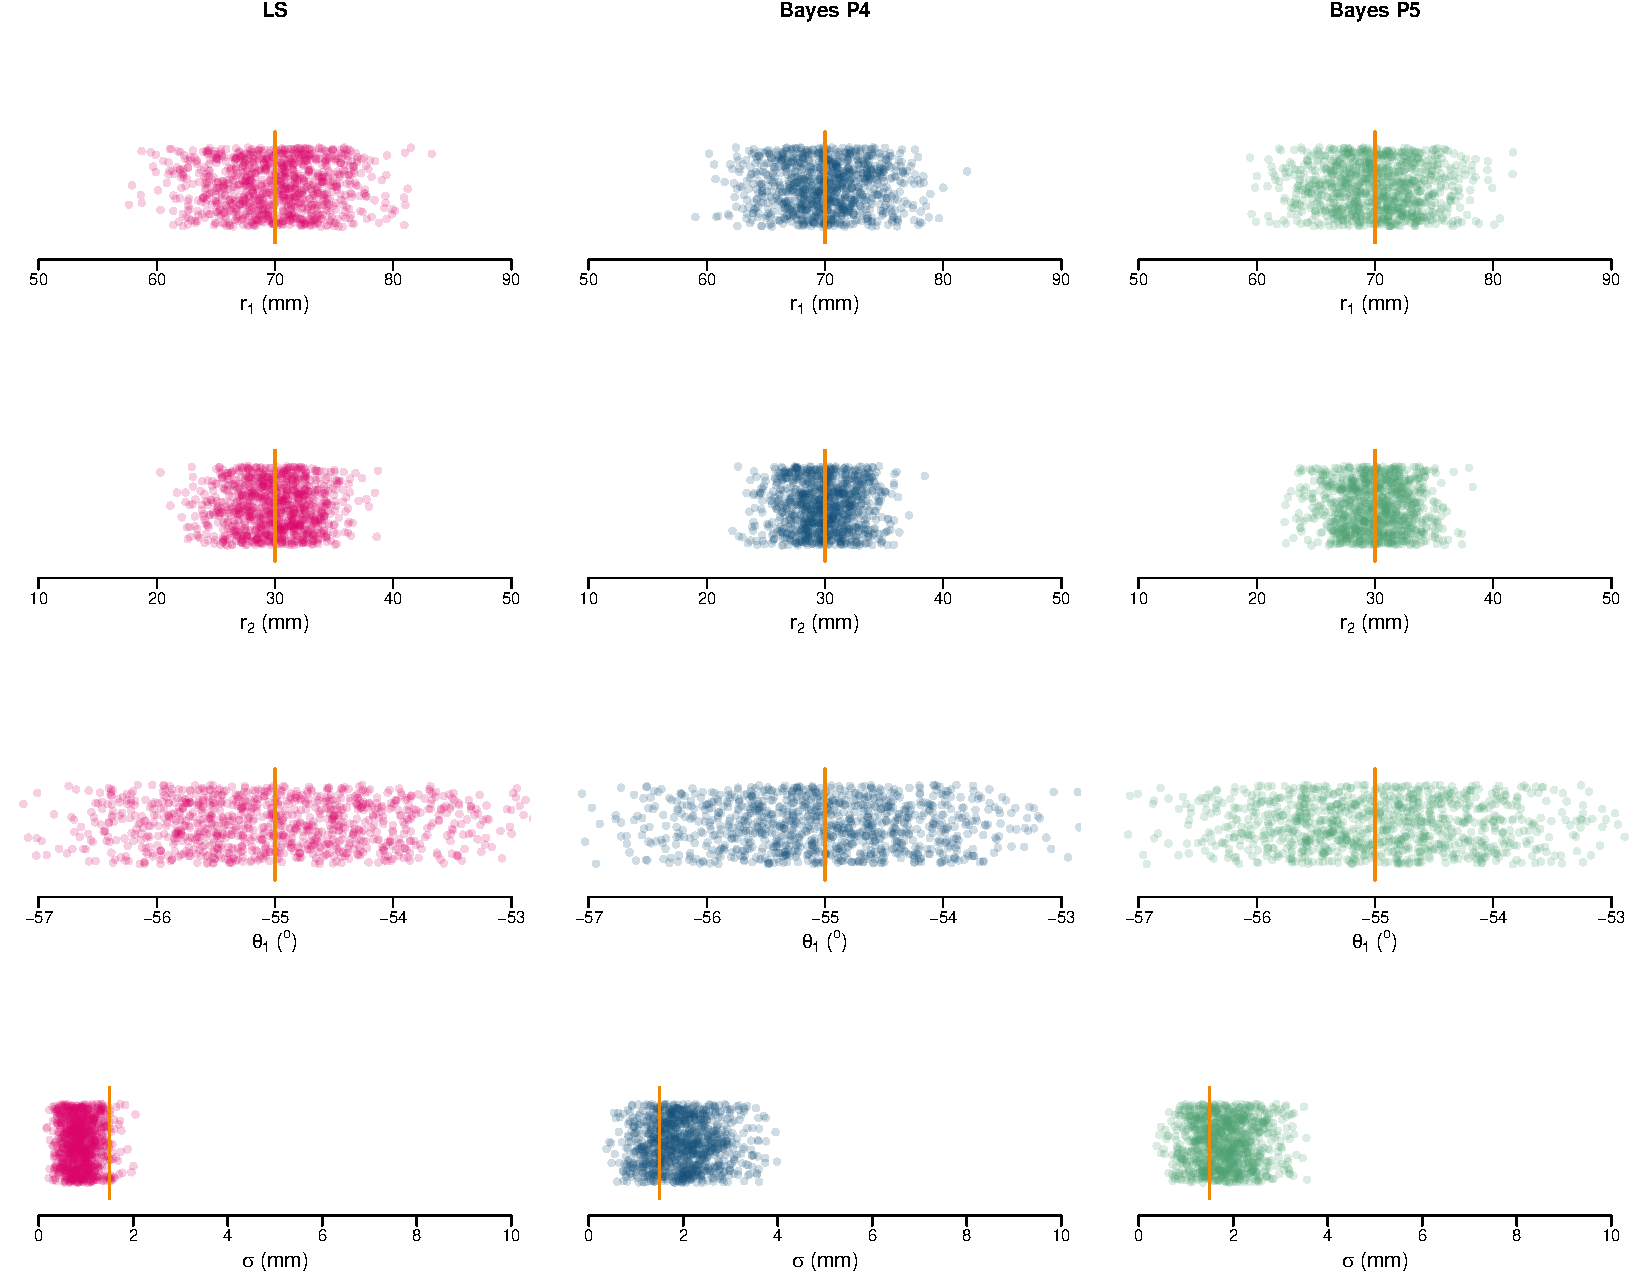
\includegraphics[width=\textwidth]{./Figures/SingleLink_StripChartP4P5.pdf}
	\caption{Performance of the estimators from models with Prior 4 and Prior 5 (columns 2 and 3) and the LS estimator (column 1) on each parameter (rows) for 1000 single link simulations.  True values for each parameter identified in orange.}
	\label{fig:StripChart_SingleLink_P4P5}
\end{figure}

\begin{figure}
	\centering
	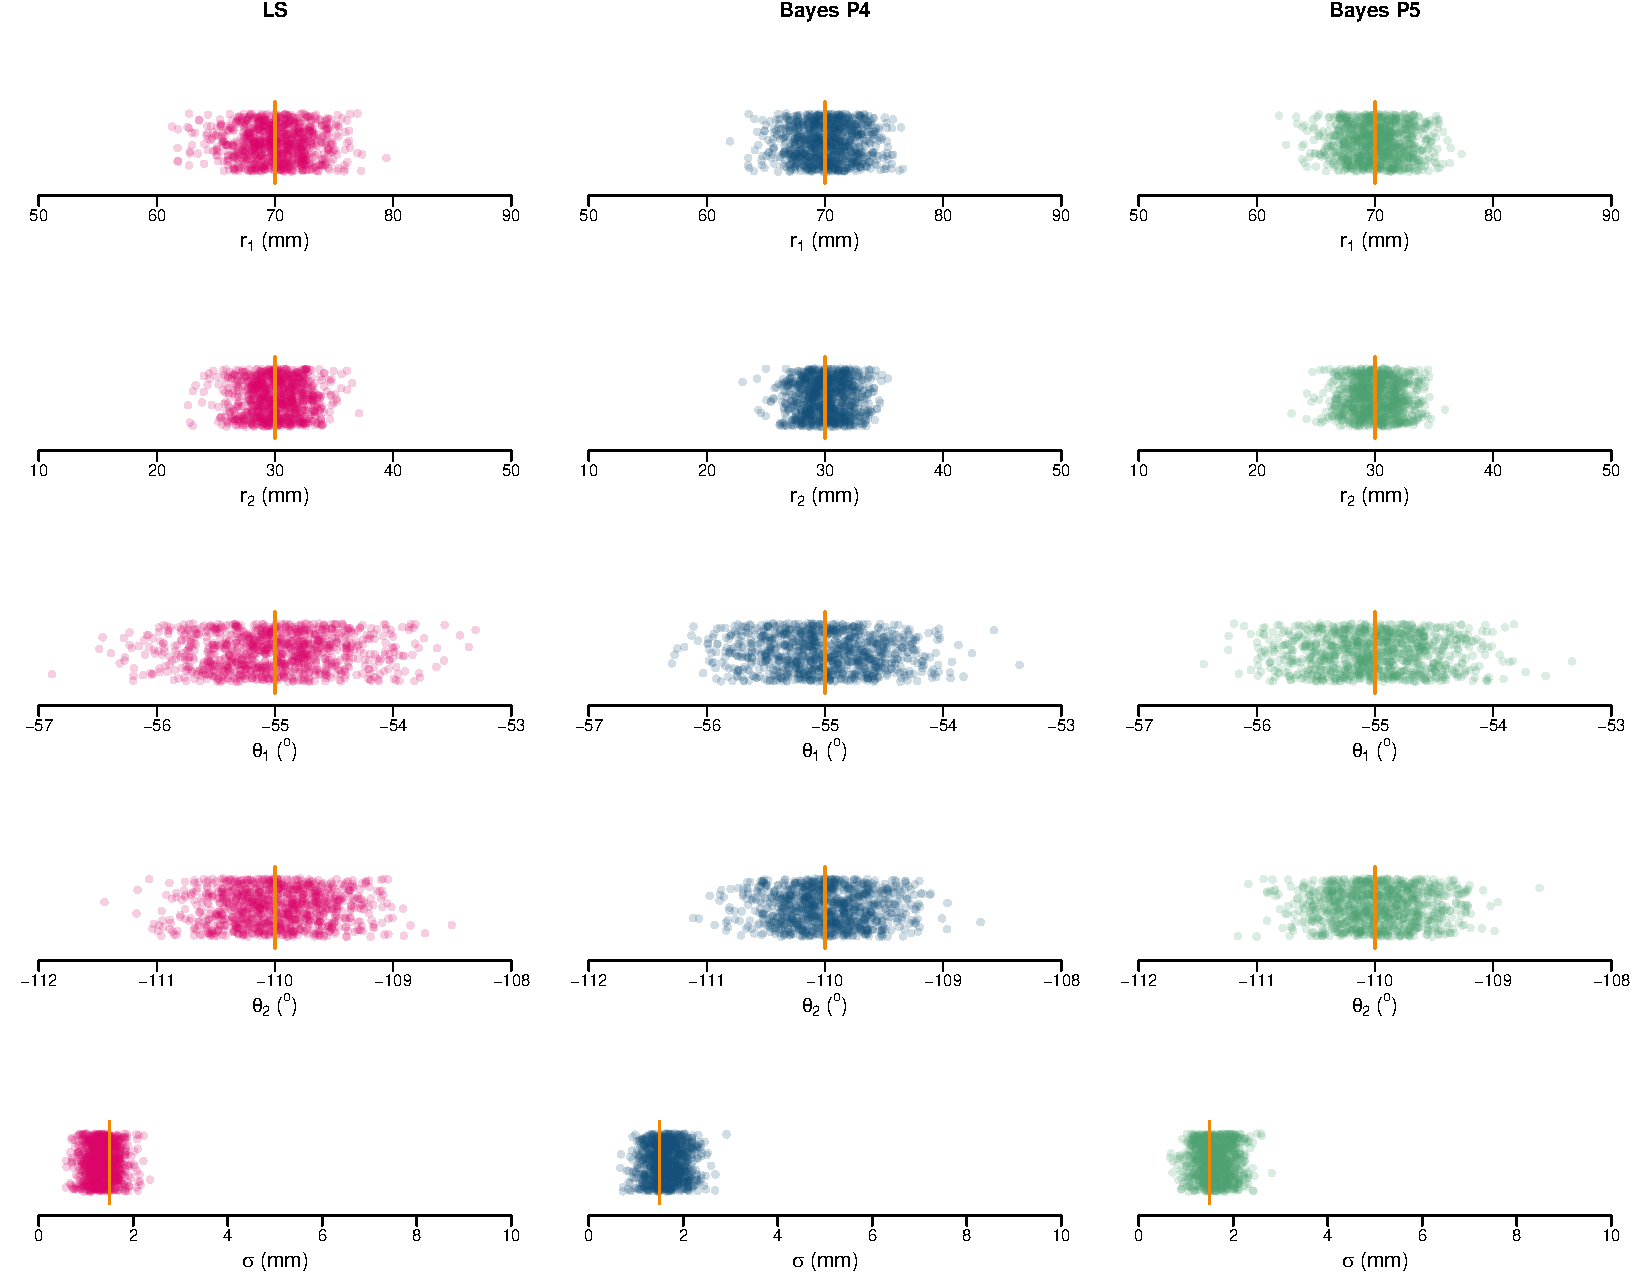
\includegraphics[width=\textwidth]{./Figures/DoubleLink_StripChartP4P5.pdf}
	\caption{Performance of the estimators from models with Prior 4 and Prior 5 (columns 2 and 3) and the LS estimator (column 1) on each parameter (rows) for 1000 double link simulations.  True values for each parameter identified in orange.}
	\label{fig:StripChart_DoubleLink_P4P5}
\end{figure}

\begin{figure}
	\centering
	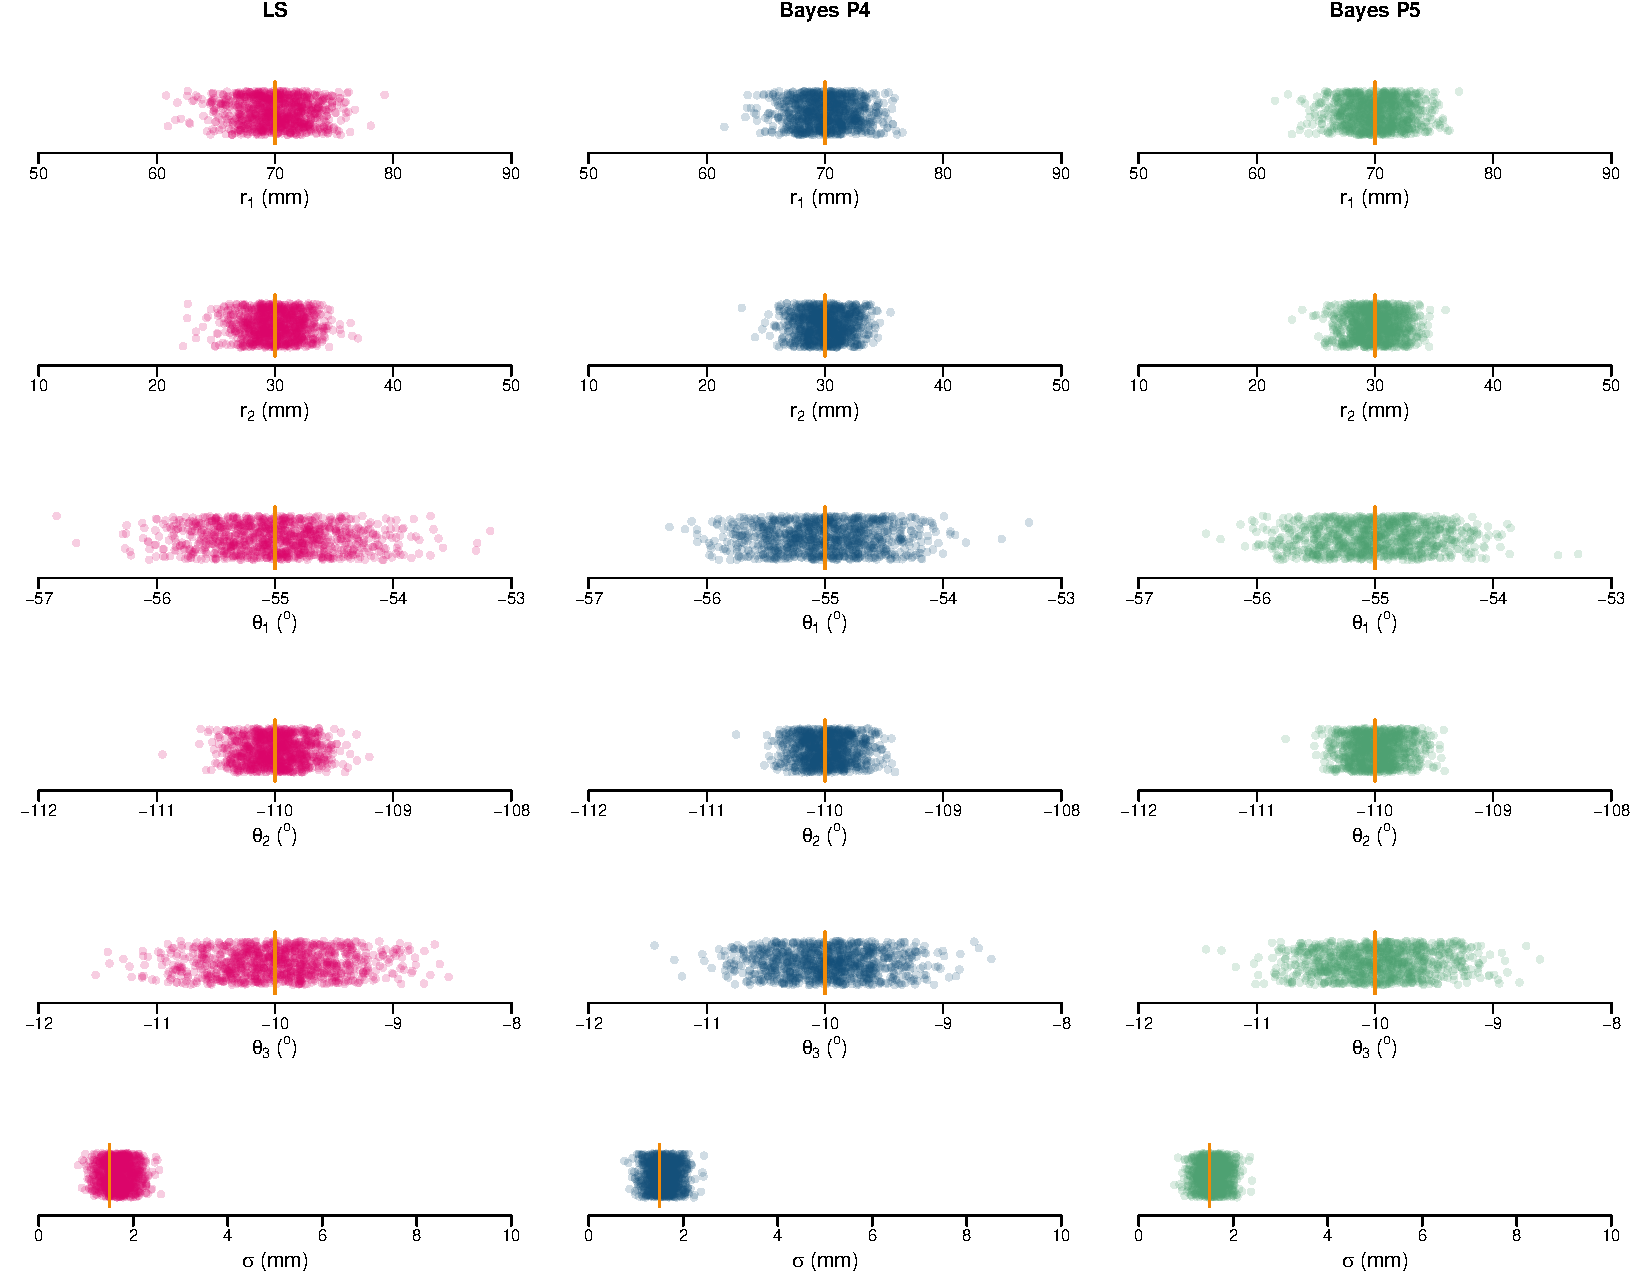
\includegraphics[width=\textwidth]{./Figures/TripleLink_StripChartP4P5.pdf}
	\caption{Performance of the estimators from models with Prior 4 and Prior 5 (columns 2 and 3) and the LS estimator (column 1) on each parameter (rows) for 1000 triple link simulations.  True values for each parameter identified in orange.}
	\label{fig:StripChart_TripleLink_P4P5}
\end{figure}

Finally, confirmation is made by examining bias, variance and RMSE of the estimators provided by models using priors 4 and 5 outlined in table \ref{tab:BiasVarianceRMSE}.  These are extremely similar to those in table 1 of the main text.  

\begin{table}[h]
	\centering
	\resizebox{\textwidth}{!}{%
		\begin{tabular}{ll cccc cccc}
			\hline
			&& & \multicolumn{3}{c}{Bayes P4} && \multicolumn{3}{c}{Bayes P5} \\
			&& & Bias & Variance & RMSE && Bias & Variance & RMSE \\
			\hline
			\multirow{4}{*}{Single Link}  && $r_1 \, (\si{\milli\meter})$ & 0.020 & 12.854 & 3.585 &&
			-0.001 & 14.352 & 3.788 \\
			&& $r_2\, (\si{\milli\meter})$ & -0.104 & 6.648 & 2.581 &&
			-0.067 & 7.328 & 2.708 \\
			&& $\theta_1 \, (^{\circ})$ & 0.009 & 0.606 & 0.778 &&
			 0.008 & 0.677 & 0.823 \\
			&& $\sigma\, (\si{\milli\meter})$ & 0.465 & 0.421 & 0.798 &&
			0.317 & 0.326 & 0.653 \\
			\hline
			\multirow{5}{*}{Double Link}  && $r_1 \, (\si{\milli\meter})$ &  
			0.086 & 5.420 & 2.330 &&
			0.080 & 5.541 & 2.355 \\
			&& $r_2\, (\si{\milli\meter})$ & 0.034 & 3.561 & 1.887 &&
			0.033 & 3.635 & 1.907\\
			&& $\theta_1\, (^{\circ})$ & -0.017 & 0.201 & 0.449 &&
			-0.016 & 0.207 & 0.455 \\
			&& $\theta_2\, (^{\circ})$ & 0.014 & 0.127 & 0.356 &&
			0.012 & 0.128 & 0.359 \\
			&& $\sigma\, (\si{\milli\meter})$ & 0.140 & 0.111 & 0.361 &&
			0.111 & 0.102 & 0.338 \\
			\hline
			\multirow{6}{*}{Triple Link}  && $r_1\, (\si{\milli\meter})$ & 0.068 & 5.209 & 2.283 &&
			0.061 & 5.337 & 2.311 \\
			&& $r_2\, (\si{\milli\meter})$ & 0.022 & 3.248 & 1.802 &&
			0.018 & 3.326 & 1.824 \\
			&& $\theta_1\, (^{\circ})$ & -0.012 & 0.184 & 0.429 &&
			-0.011 & 0.189 & 0.435 \\
			&& $\theta_2\, (^{\circ})$ & 0.008 & 0.038 & 0.196 &&
			0.008 & 0.039 & 0.197 \\
			&& $\theta_3\, (^{\circ})$ & 0.013 & 0.166 & 0.408 &&
			0.014 & 0.170 & 0.413 \\
			&& $\sigma\, (\si{\milli\meter})$ & 0.084 & 0.067 & 0.272 &&
			0.067 & 0.063 & 0.261 \\
			\hline
		\end{tabular}
	}
	\caption{Bias, Variance and RMSE of estimators for each model on one, two and three link simulations when the LS solution is used as initial conditions for MCMC computation and true values used as initial conditions for numerical optimisation with respect to the LS estimator.}
	\label{tab:BiasVarianceRMSE}
\end{table}

The same can be said for the proportion of iterations in which models using prior 4 or prior 5 had lower absolute error than the LS estimator with LS prior Bayesian models outperforming the LS estimator between 52 and 69\% of iterations (table 2).  This is similar to what were observed for vague and weakly-informative priors in the main text.

\begin{table}
	\centering
	%\resizebox{}{!}{%
	\begin{tabular}{l l c c c c c c}
		\hline
		Model & Pose & $r_1$ & $r_2$ & $\theta_1$ & $\theta_2$ & $\theta_3$ & $\sigma$\\
		\hline
		\multirow{3}{*}{Bayes P4} & 1 - Link & 59.8 & 61.2 & 60.5 & - & - & 58.2\\
		& 2 - Link & 57.0 & 56.5 & 59.2 & 60.5 & - & 52.5\\
		& 3 - Link & 58.3 & 60.3 & 59.7 & 58.8 & 59.1 & 69.0\\
		\hline
		\multirow{3}{*}{Bayes P5} & 1 - Link & 62.6 & 63.3 & 62.7 & - & - & 65.4\\
		& 2 - Link & 57.0 & 58.4 & 61.7 & 60.9 & - & 55.8\\
		& 3 - Link & 59.4 & 60.1 & 61.4 & 59.2 & 59.9 & 67.8\\
		\hline

	\end{tabular}
	%}
	\caption{Percentage of simulations in which Bayesian estimator had lower absolute error than the MLE when the LS solution was used to initialise MCMC sampling. The equivalent results using random values for initial conditions can be found in table 1 in Appendix B}
	\label{tab:PerformanceTrueVals}
\end{table}

\section{Discussion}
Beyond the experimental findings presented above a theoretical argument can be made to suggest that models with LS centred priors will not drastically outperform the LS estimator.  If increasingly informative priors are constructed centred on the LS solution then the posterior will converge to the LS solution as the informative nature of the marginal prior converges to a point mass distribution for the respective parameter.  For example, as the standard deviation in the normal distributions used for the informative LS centred prior (prior 5) tends to 0, then the resulting prior distribution resembles a point mass and as a result the posterior distribution will also resemble a point mass at the LS solution.  At the other extreme as the standard deviation increases towards infinity then the prior distribution resembles a flat, non-informative prior.


\bibliography{References.bib}

\end{document}
